%======================================================================
\subsection{UI step C plan: structure (21 Oct 2026, approved 22 Oct)}\label{sec:ui-stepC}
%======================================================================

Step C is the part of the UI work that changes how the window is organised. Steps A and B left that alone.
This section is the plan for it, written to be approved before any of it is built (your rule for big
features). It covers five items, figure~\ref{fig:stepC-bar}:
\begin{enumerate}[nosep,label=\textbf{C\arabic*}]
  \item Captioned tool groups (\eref{UIX-06}).
  \item The workspace menu and its tabs, with Fusion naming (\eref{UIX-05}).
  \item Search, read as a built-in \texttt{Cmd-K} field (\eref{UIX-06}; your ``yes'' from the second round, still to be confirmed).
  \item Document tabs in the macOS title bar (\eref{UIX-06}).
  \item The Start page (\eref{UIX-06}, \eref{PDM-04}).
\end{enumerate}
The Browser badges were listed under step C in the plan table of section~\ref{sec:ui-design}. They moved into step B
(item 7, being built tonight), so they are not repeated here. Nothing in this section is built yet. The two
prototypes in figure~\ref{fig:stepC-proto} are throw-away feasibility checks, kept in the agents' scratch folder.

\begin{figure}[!htbp]
\centering
\begin{tikzpicture}
  \node[anchor=south west,inner sep=0] (img) at (0,0) {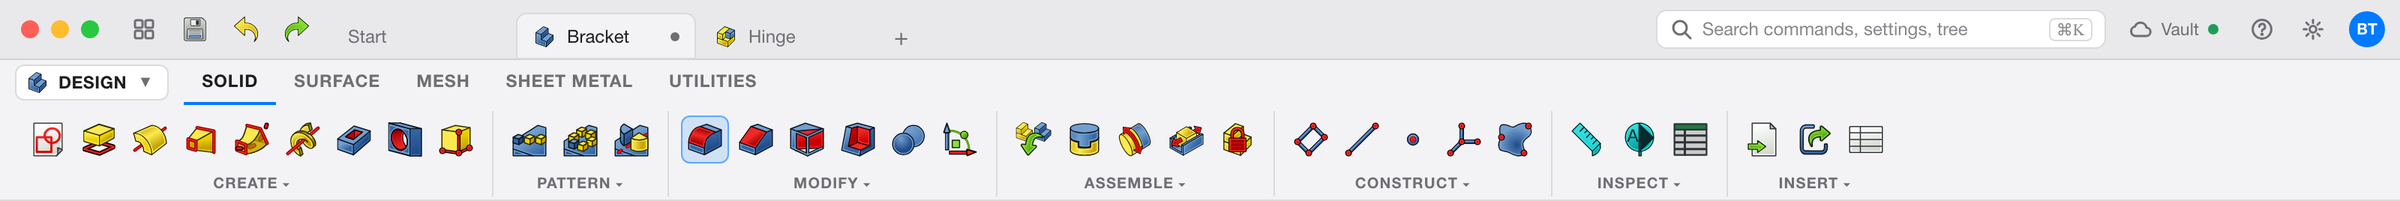
\includegraphics[width=\linewidth]{fig/ui_stepC_bar.png}};
  \begin{scope}[x={(img.south east)},y={(img.north west)}]
    \foreach \n/\x/\y in {C4/0.138/0.80, C3/0.677/0.80, C2/0.093/0.57, C2/0.335/0.57, C1/0.160/0.10}
      \node[circle,fill=bwred,text=white,font=\tiny\bfseries,inner sep=0.6pt,minimum size=13pt,draw=white,line width=0.8pt] at (\x,\y) {\n};
  \end{scope}
\end{tikzpicture}
\caption{The top of the window in the mock (part modelling, light), with the step C items marked. Document tabs
and search sit in the title bar (C4, C3). Below them are the workspace menu and its tabs (C2), then the captioned
groups (C1).}
\label{fig:stepC-bar}
\end{figure}

\paragraph{One idea runs through all five: build it in Python, on stock FreeCAD.}
Everything below is planned as Python modules in \file{src/Mod/BruceWorx/}, like steps A and B. They use
FreeCAD's own extension points: custom toolbars, workbench manipulators, document observers, and the
\code{StartView}'s page stack. Each module gets a switch on Preferences $\rightarrow$ BruceWorx, on by default.
Turning a switch off gives back the stock window. The reason is the planned rebase onto upstream \code{main}
(\S\ref{sec:asm-audit}). A Python module in our own folder cannot conflict with upstream, but every
\code{[BW]} line in \file{src/Gui} can. \file{MainWindow.cpp} already carries about 390 \code{[BW]} lines after
tonight's step B work. Where C++ would be cleaner, the alternative is named, with the reason not to choose it
first.

Line numbers below are from the working tree on 21 Oct 2026, 14:00. Other agents edit some of these files, so
the numbers may move by a few lines.

%----------------------------------------------------------------------
\subsubsection*{C1. Captioned tool groups}

\textbf{What you see.} Every tool group on the toolbar row has a small caption under it: \textsc{Create},
\textsc{Pattern}, \textsc{Modify} and so on. All icons are 24\,px. Clicking a caption opens a menu with every
command in the group, named, including those that do not fit on the row (figure~\ref{fig:stepC-groups}, left). No
icon is redrawn.

\textbf{How it is built.}
\begin{itemize}[nosep]
  \item \emph{Caption.} A module \file{bruceworx\_groups.py} gives each workbench toolbar in the top area a bottom
        contents margin of 14\,px. It then places a flat child \code{QToolButton} (caption text and
        $\blacktriangledown$) in that strip, centred under the buttons. An event filter on \code{Resize} and
        \code{LayoutRequest} keeps the button in place. \code{QToolBar}'s size hint includes the margin, so the
        row grows by itself. This was checked tonight with Qt~6.8.3 offscreen, using FreeCAD's icons
        (figure~\ref{fig:stepC-proto}, top): toolbar height $31 + 14 = 45$\,px, as computed.
  \item \emph{Menu.} The caption's \code{QMenu} holds the toolbar's own \code{QAction}s. These are the same objects,
        so enabled state, checked state and shortcuts stay live without any syncing. Commands that the
        workspace definition (C2) lists as ``more in this group'' are added below a separator.
  \item \emph{Icon size.} \code{ToolBarManager} reads \code{General/ToolbarIconSize}, default 24
        (\file{ToolBarManager.cpp:474}). The pack sets it to 24. The group dividers and the caption type
        (10\,px semibold capitals) go in \file{BruceWorx.qss}.
  \item \emph{App toolbars} (File, View, Edit, Macro: the \code{APP\_TOOLBARS} list in
        \file{bruceworx\_toolbars.py}) get no caption. C4 moves most of them into the title row anyway.
\end{itemize}
\emph{C++ alternative:} paint the caption in \code{Gui::ToolBar} (\file{ToolBarManager.h:125}) by overriding
\code{paintEvent} and \code{sizeHint}. This is cleaner, but every toolbar in FreeCAD would then carry a
\code{[BW]} change. Keep it in reserve in case the Python child button misbehaves when toolbars are dragged or
floated.

\textbf{Effort:} 1--2 days. \textbf{Risks:} A floating or vertical toolbar must drop its caption (the margin is
set only for the top area). Toolbars should be locked in the top area while the Vector Labs bar is on
(\code{ToolBarManager::setToolBarsLocked}), otherwise a drag can land a group in a second row with its caption
cut off. No upstream conflict.

\begin{figure}[!htbp]
\centering
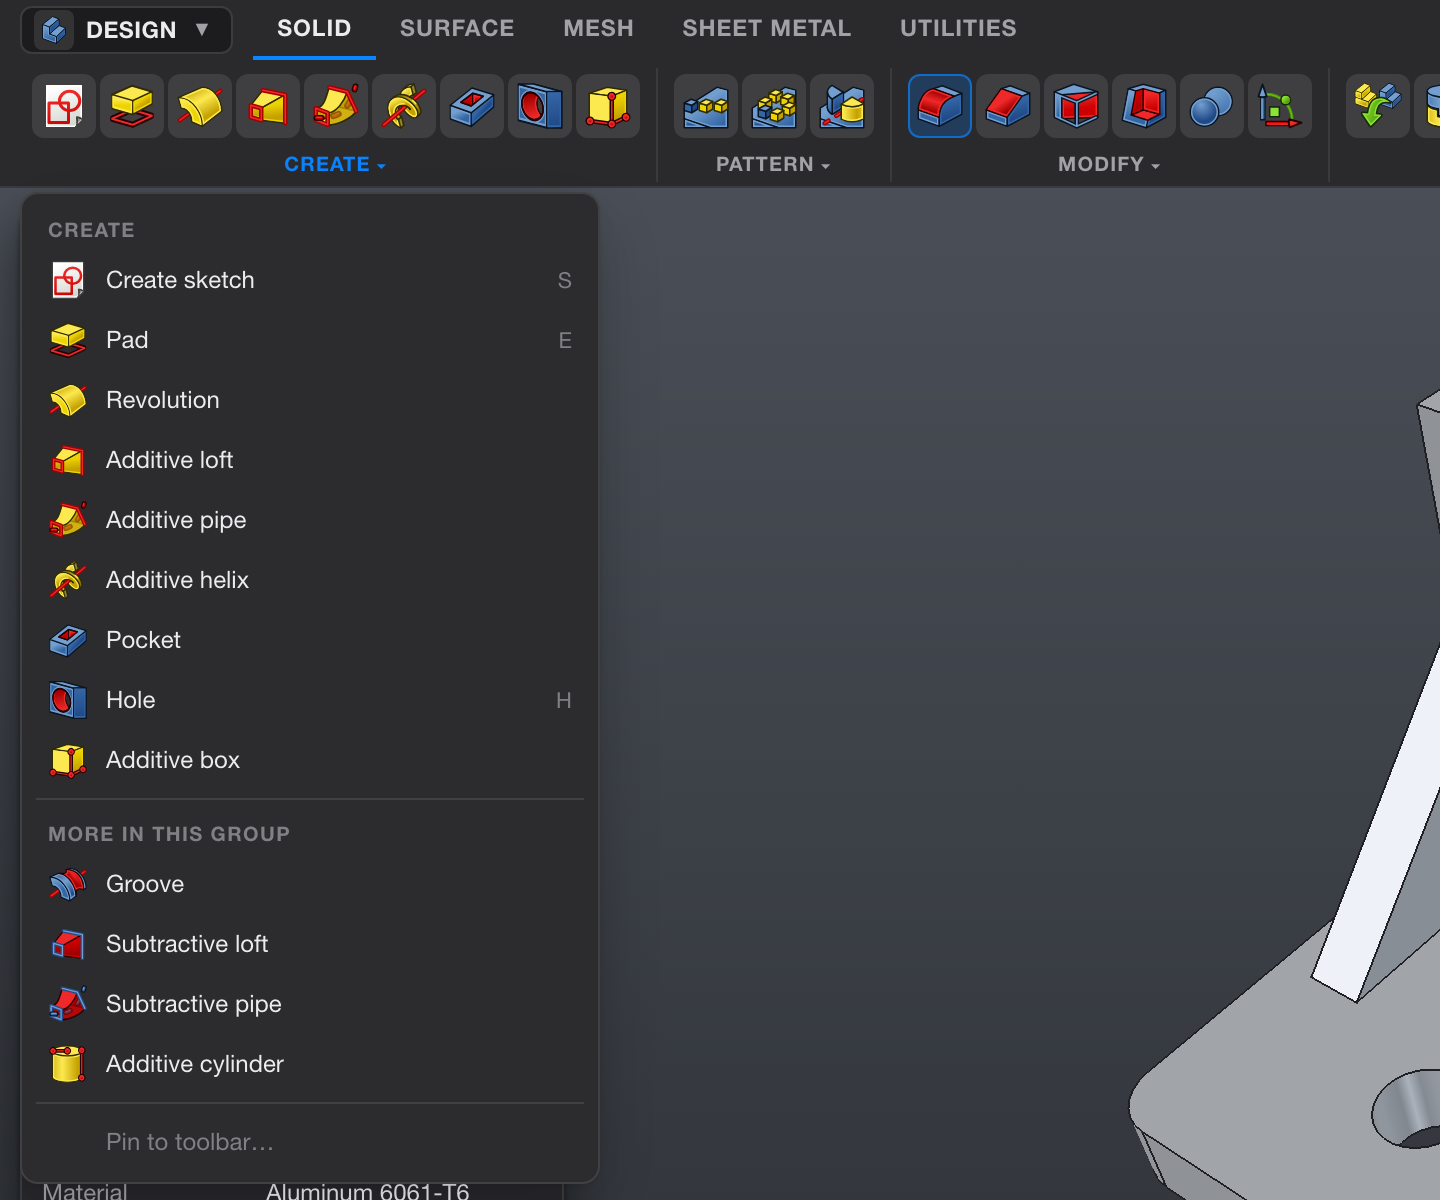
\includegraphics[width=0.497\linewidth]{fig/ui_stepC_groups.png}\hfill
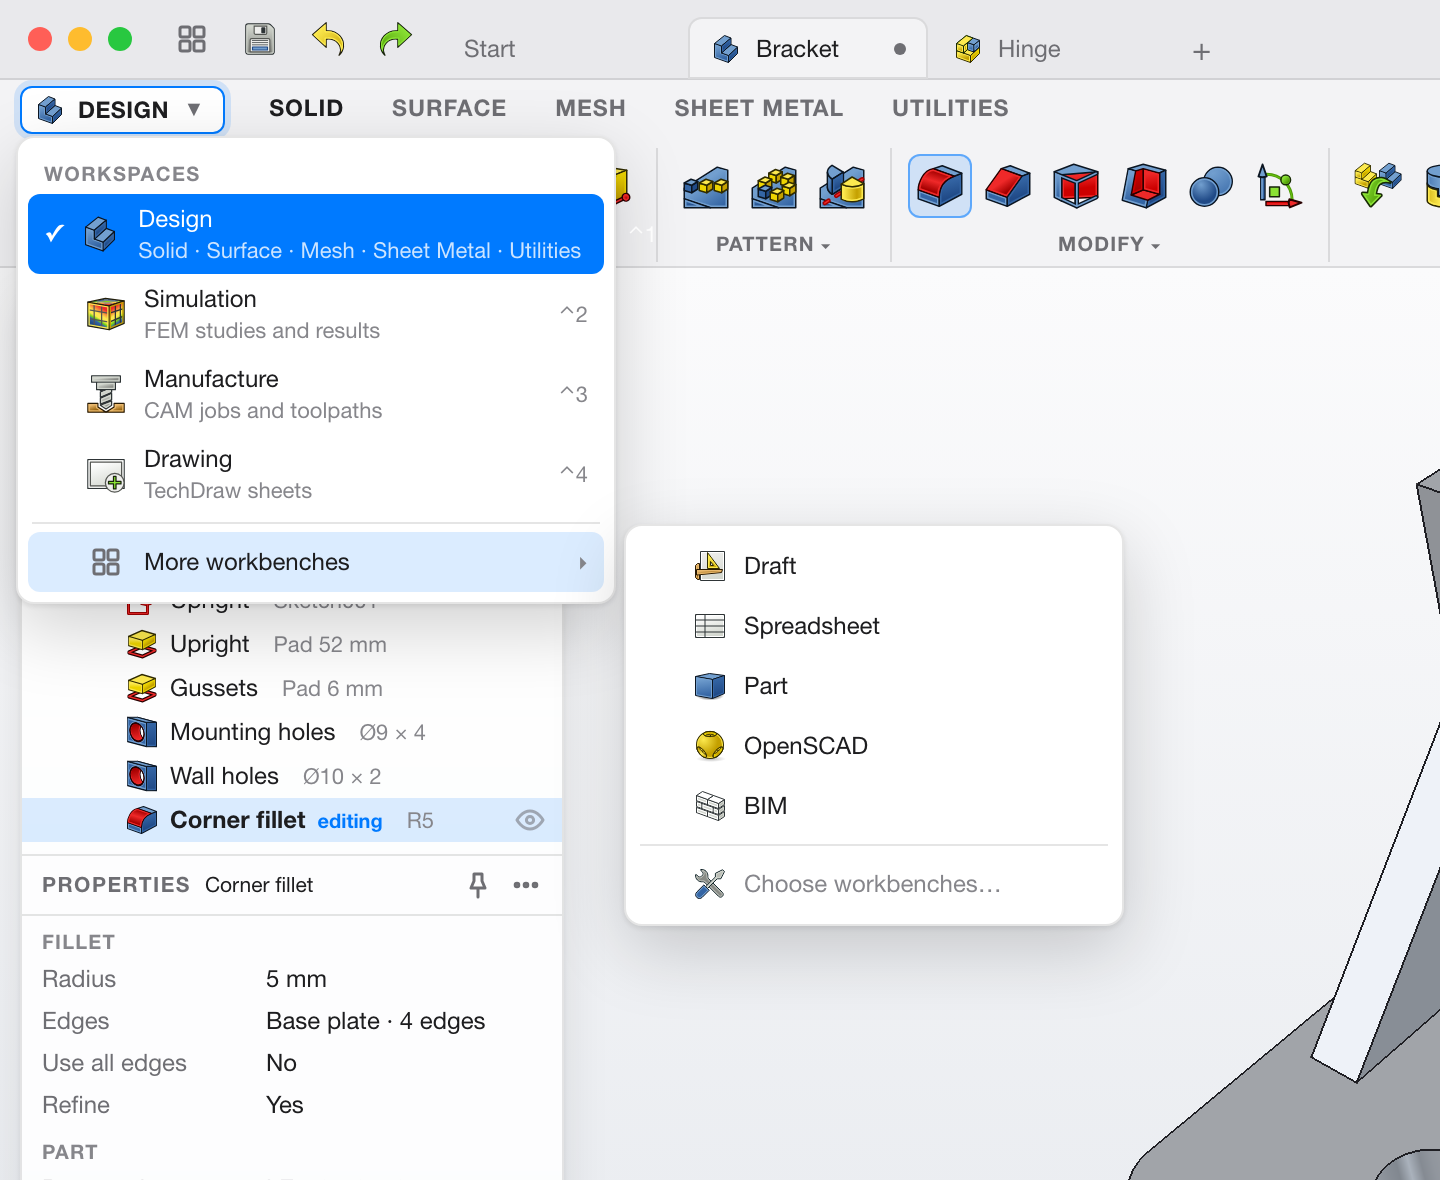
\includegraphics[width=0.497\linewidth]{fig/ui_stepC_ws.png}
\caption{\emph{Left (C1, dark):} the \textsc{Create} caption opened. The row's nine commands come first, with
shortcuts. Then come four more Create commands that do not fit on the row. \emph{Right (C2, light):} the
workspace menu, with \emph{More workbenches} open. The four workspaces have \texttt{Ctrl-1}\ldots\texttt{4}. The
submenu lists only the workbenches ticked in Preferences.}
\label{fig:stepC-groups}
\end{figure}

%----------------------------------------------------------------------
\subsubsection*{C2. Workspace menu and tabs (Fusion naming)}

\textbf{What you see.} The \textsc{Design} button opens the menu in figure~\ref{fig:stepC-groups} (right). It lists
the four workspaces and a \emph{More workbenches} submenu. Design has the tabs \textsc{Solid},
\textsc{Surface}, \textsc{Mesh}, \textsc{Sheet Metal} and \textsc{Utilities}. Opening a sketch adds a
\textsc{Sketch} tab in the accent colour and switches to it. \textsc{Finish Sketch} closes the tab again
(figure~\ref{fig:stepC-sketch}). Choosing a workbench from \emph{More} shows that workbench's own toolbars as
captioned groups under a single tab with its name.

\begin{figure}[!htbp]
\centering
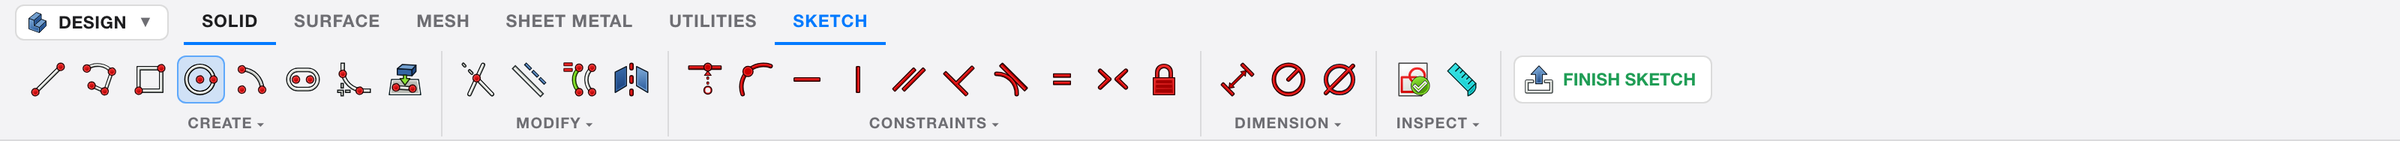
\includegraphics[width=\linewidth]{fig/ui_stepC_sketchtab.png}
\caption{C2: the contextual \textsc{Sketch} tab while a sketch is open (from figure~\ref{fig:ui-sketch-start}).}
\label{fig:stepC-sketch}
\end{figure}

\textbf{Model (from the starting brief).} A workspace $w$ fixes one FreeCAD workbench $\beta(w)$. A tab $t$
fixes a set of toolbars $\tau(w,t)$, the ones shown while the tab is open:
\begin{center}
\small
\begin{tabular}{@{}lll@{}}
\toprule
Workspace $w$ & Workbench $\beta(w)$ & Tabs\\
\midrule
Design & \code{PartDesignWorkbench} & Solid, Surface, Mesh, Sheet Metal, Utilities; contextual Sketch\\
Simulation & \code{FemWorkbench} & one tab to start (question~4)\\
Manufacture & \code{CAMWorkbench} & one tab to start\\
Drawing & \code{TechDrawWorkbench} & one tab\\
\bottomrule
\end{tabular}
\end{center}
Changing workspace calls \code{Gui.activateWorkbench}. That is FreeCAD's normal workbench switch, with its
toolbar and menu rebuild. Changing tabs inside a workspace only shows and hides toolbars. There is no rebuild,
so there is no flicker.

\textbf{How it is built.}
\begin{itemize}[nosep]
  \item \emph{Definition.} A data file \file{workspaces.json} in the module gives, for each workspace, its workbench, its
        tabs, each tab's groups (caption plus command names), and the ``more'' commands. One file is easy to
        review and diff, and a test can check that every command named in it exists.
  \item \emph{Groups made from several workbenches.} A Python manipulator cannot add a new toolbar.
        \code{append} only adds to a toolbar that already exists (\file{WorkbenchManipulatorPython.cpp:296--306}).
        FreeCAD's \emph{custom toolbars} can, though. At every activation, \code{Workbench::activate} reads
        \code{BaseApp/Workbench/<wb>/Toolbar/*} (\file{Workbench.cpp:452}, \file{256--330}). For a command
        that is not registered yet, it imports the module named in the entry, then that name plus
        \code{Gui}. That is exactly the cross-workbench loading Design needs: Assembly joints, Part booleans,
        Surface, Mesh and SheetMetal commands inside \code{PartDesignWorkbench}. At start-up,
        \file{bruceworx\_workspaces.py} writes one custom toolbar per group, \code{BW\_Solid\_Create} with
        \code{Name = "Solid · Create"} and so on. It first removes its own old \code{BW\_*} groups, so the result is
        always fresh and nothing the user customised is touched. The stock toolbars of $\beta(w)$ are taken
        out with the manipulator's \code{remove} (\file{WorkbenchManipulatorPython.cpp:308--330}) while the
        bar is on.
  \item \emph{The bar.} It is one \code{QToolBar} named \code{BruceWorxWorkspaces}: a menu button plus a
        \code{QTabBar}. Its \code{toggleViewAction} is hidden, so \code{ToolBarManager::setup} leaves it alone
        on every switch (\file{ToolBarManager.cpp:772--786} only hides toolbars whose toggle action is
        visible). The stock \emph{Workbench} toolbar, made by \code{WorkbenchGroup::addTo}
        (\file{Action.cpp:655--670}), is hidden while the bar is on.
  \item \emph{Tab switch.} The bar shows the toolbars in $\tau(w,t)$ and hides the rest. The last tab used in
        each workspace is kept in \code{BruceWorx/Workspaces/<w>/Tab}. \code{ToolBarManager} restores the
        saved visibility on every activation, so the bar applies the tab again after
        \code{workbenchActivated}, deferred with a zero-length timer the way \file{bruceworx\_toolbars.py} does
        it today. That module's two-row relayout becomes part of this one.
  \item \emph{Contextual Sketch tab.} Sketcher already force-shows its edit toolbars on entering a sketch and
        hides them on leaving (\code{Sketcher::Workbench::enterEditMode}, \file{Sketcher/Gui/Workbench.cpp:205},
        \code{leaveEditMode} \file{:225}; toolbar names at \file{:156--167}). The bar listens to the same moment
        through a GUI document observer (\code{slotInEdit} and \code{slotResetEdit},
        \file{DocumentObserverPython.cpp:237, 251}). It pushes or pops a \textsc{Sketch} tab whose groups are
        those toolbars, captioned \textsc{Create}, \textsc{Modify}, \textsc{Constraints} and
        \textsc{Dimension}, with \code{Sketcher\_LeaveSketch} as \textsc{Finish Sketch}.
  \item \emph{More workbenches and Preferences.} FreeCAD already keeps the list of enabled and disabled workbenches
        (\code{DlgSettingsWorkbenchesImp::getEnabledWorkbenches}/\code{getDisabledWorkbenches},
        \file{PreferencePages/DlgSettingsWorkbenchesImp.cpp:467, 509}). A disabled workbench is never loaded.
        The submenu shows the enabled ones that are not one of the four. The BruceWorx preference page gets a
        \emph{Workspaces} section (figure~\ref{fig:stepC-prefs}) that writes that same stock list, so there
        is one source of truth (question~5).
\end{itemize}
\emph{C++ alternative (the starting brief's):} a \code{WorkspaceSelector} as selector type~2 in
\code{WorkbenchGroup::addTo} (\file{Action.cpp:664}), next to \code{WorkbenchComboBox} and
\code{WorkbenchTabWidget} (\file{WorkbenchSelector.h:48, 68}). It would show up in the stock Workbenches
preference page. However, it touches two upstream files that change often, and it does not need anything that
Python lacks. It is not recommended unless the Python bar proves too slow (question~2).

\textbf{Effort:} 3--4 days, the largest item. \textbf{Risks:}
\begin{itemize}[nosep]
  \item \emph{Commands outside their own workbench.} Most only check the document (an Assembly joint needs an
        active assembly). The Assembly workbench's task watchers (\file{Mod/Assembly/InitGui.py},
        \code{Activated}) and its context menu do not come along. The manipulator's \code{modifyContextMenu}
        can add the Assembly items when an assembly is active. Question~3 asks whether an assembly document
        should switch $\beta$ to Assembly instead.
  \item \emph{Sheet Metal} is an add-on, so its tab is shown only when the add-on is installed (bundling it is
        in the roadmap).
  \item \emph{Custom toolbar order.} \code{GetASCIIMap} is expected to keep the command order as written.
        \verify
  \item \emph{Upstream.} No conflict, except that upstream may rename commands. The json test catches that.
\end{itemize}

\begin{figure}[!htbp]
\centering
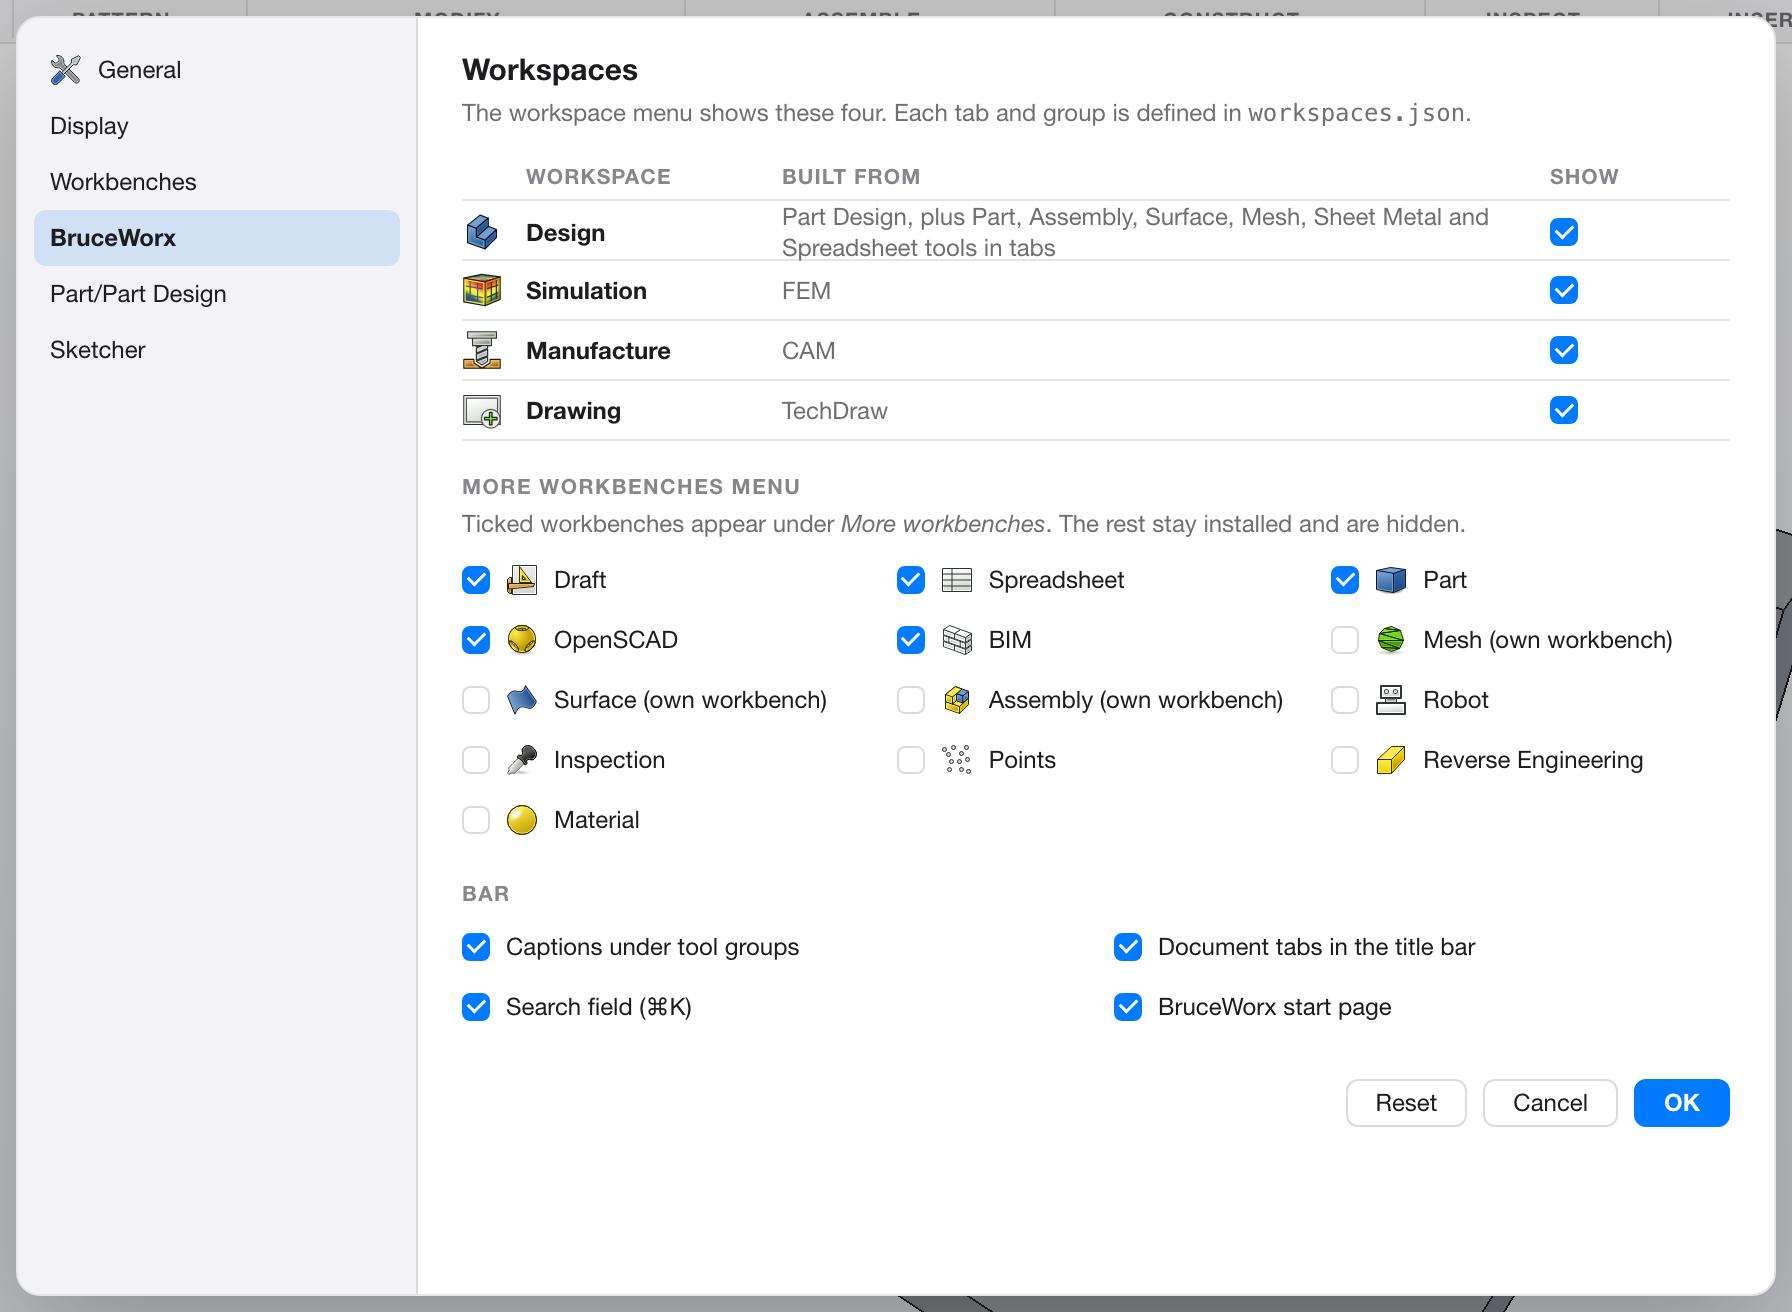
\includegraphics[width=0.78\linewidth]{fig/ui_stepC_prefs.png}
\caption{C2 and question~5: the \emph{Workspaces} section on Preferences $\rightarrow$ BruceWorx. The ticks under
\emph{More workbenches menu} write FreeCAD's own enabled/disabled workbench list. The four switches at the
bottom turn the step C items off one by one.}
\label{fig:stepC-prefs}
\end{figure}

%----------------------------------------------------------------------
\subsubsection*{C3. Search (\texttt{Cmd-K})}

\textbf{What you see.} One field in the title bar. \texttt{Cmd-K} focuses it from anywhere. Typing lists
\emph{commands} with the place they live in the workspaces, \emph{objects in this document}, and
\emph{settings} (figure~\ref{fig:stepC-search}). \texttt{Return} runs the command, selects the object, or
opens Preferences at that setting. \texttt{Cmd-Return} shows where a command lives by opening its tab and
flashing it.

\begin{figure}[!htbp]
\centering
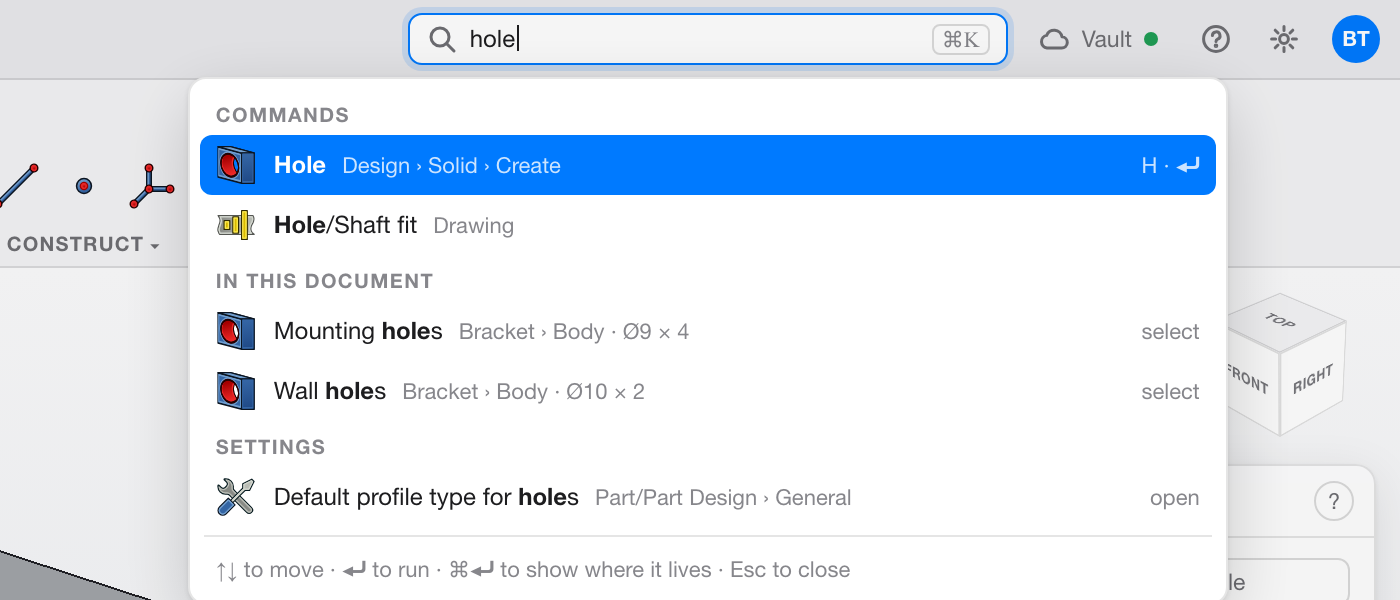
\includegraphics[width=0.497\linewidth]{fig/ui_stepC_search.png}\hfill
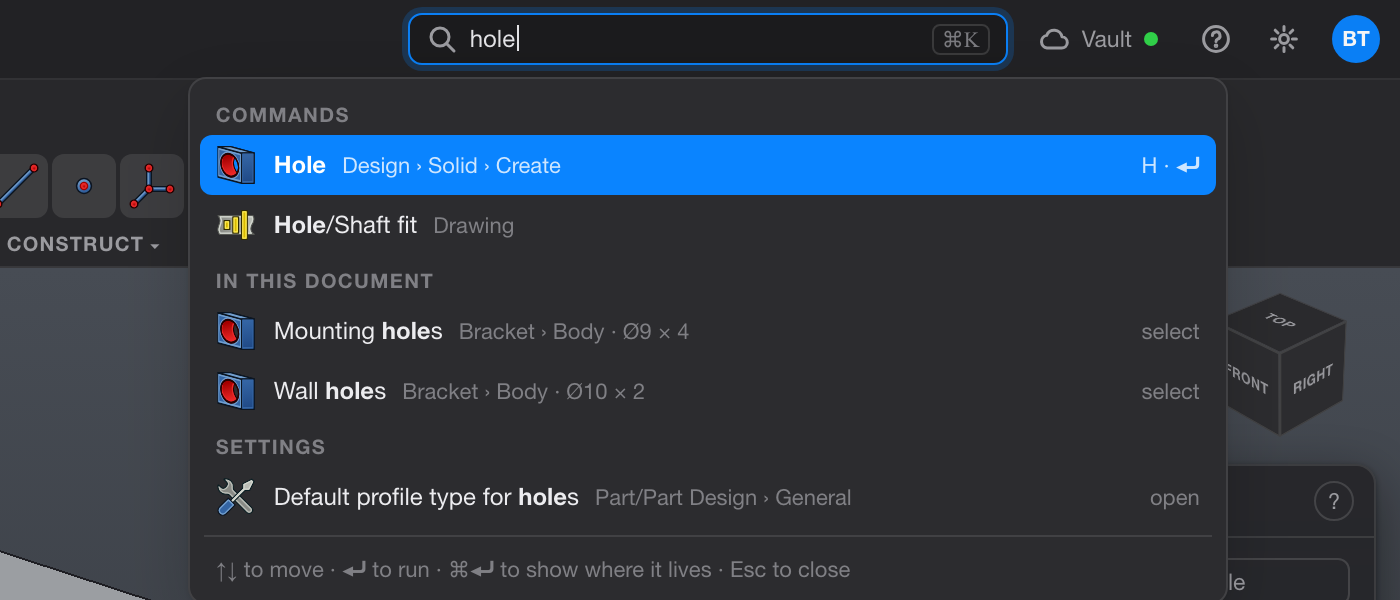
\includegraphics[width=0.497\linewidth]{fig/ui_stepC_search-dark.png}
\caption{C3: ``hole'' finds the command (with its place, \textsc{Design $\rightarrow$ Solid $\rightarrow$ Create}),
the two hole features in the open part, and a real setting (\emph{Default profile type for holes}, from
\file{Part/Gui/DlgSettingsGeneral.ui}).}
\label{fig:stepC-search}
\end{figure}

\textbf{How it is built (built-in, recommended).} A module \file{bruceworx\_search.py} provides a
\code{QLineEdit} and a pop-up list.
\begin{itemize}[nosep]
  \item \emph{Commands:} \code{Gui.Command.listAll()} and \code{getInfo()} (menu text, tooltip, icon, shortcut;
        \file{Command.pyi:35, 106}), run with \code{Command.run()}. The place in the workspaces comes from
        \file{workspaces.json}, and only active commands are listed first.
  \item \emph{Document:} labels, \code{Label2} and types of the active document's objects. A hit selects the
        object and scrolls the Browser to it.
  \item \emph{Settings:} the labels and tooltips of the preference pages' \file{.ui} files, indexed once in the
        background. A hit opens Preferences with the text in its own search box. FreeCAD 1.1 has one
        (\code{PreferencesSearchController}, \file{Dialogs/DlgPreferencesImp.h:50}).
\end{itemize}
Ranking is a subsequence match: start-of-word hits score highest, then recent use. \texttt{Cmd-K} is free: no
FreeCAD command binds \texttt{Ctrl+K}, which is \texttt{Cmd-K} on the Mac. Tree search keeps \texttt{Cmd-F}
(\file{Tree.cpp:1898}). The command index is shared with the command line (\eref{AUT-05}). Search \emph{finds}
things, and the command line \emph{types} aliases and Python.

\emph{Alternative:} bundle the SearchBar add-on (v1.8.1.1, already in your profile). It searches the same three
kinds of thing, but it brings its own toolbar, a mouse-pointer bar, a ``what changed'' dialog and a
103\,000-line \file{Resources.py}. Its \file{package.xml} says CC0 while its \file{LICENSE} is LGPL-2.1. It is
left installed. Like Ribbon, its toolbar is hidden while the BruceWorx field is on.

\textbf{Effort:} about 2 days. \textbf{Risks:} Settings search depends on stock dialog internals, so it falls
back to just opening Preferences. A large document needs the object list cached per recompute. No upstream
conflict.

%----------------------------------------------------------------------
\subsubsection*{C4. Document tabs in the macOS title bar}

\textbf{What you see.} The mock's top row (figure~\ref{fig:stepC-bar}). The traffic lights, then save, undo and
redo, then the document tabs (modified dot instead of $\times$, $\times$ on hover), then search, vault state and
help on the right. There is no separate title strip, which gives back 28--40\,px of height. Dragging any empty
part of the row moves the window, and double-clicking it zooms, as in any Mac app. Step B (tonight) puts the tabs
in a row under the title bar. That stays as the fallback you already accepted (answer~6) and as the layout on
other platforms.

\textbf{How it is built.}
\begin{enumerate}[nosep]
  \item \emph{Window.} The window's \code{NSWindow} gets \code{styleMask |= NSWindowStyleMaskFullSizeContentView}
        ($2^{15}$), \code{titlebarAppearsTransparent = YES} and \code{titleVisibility = NSWindowTitleHidden}. The
        Qt content then runs under the traffic lights. Qt's unified title and toolbar is switched off for this,
        because the two would fight (\code{MainWindow::applyMacUnifiedTitleBar},
        \file{MainWindow.cpp:1383--1398}).
  \item \emph{Safe area.} Found by the prototype: Qt~6.8 keeps the old title strip as a \emph{safe area}, and
        its layouts stay below it, so the row first landed 28\,pt down (figure~\ref{fig:stepC-proto}). Setting
        \code{Qt::WA\_ContentsMarginsRespectsSafeArea} to false on the main window (\file{qnamespace.h:416} of
        this Qt) puts the row at $y = 0$, which was checked.
  \item \emph{The row.} It is a non-movable top toolbar \code{BruceWorxTitleRow}, on the first line, with its
        toggle action hidden as in C2 and a left inset for the traffic lights (about 78\,pt). Its tab bar mirrors
        the MDI area's sub-windows (\code{QMdiArea::subWindowActivated}, window titles and modified state),
        and the MDI area's own tab bar is hidden. Step B's tab button with the modified dot
        (\code{DocumentTabButton} in \file{MainWindow.cpp}) is reused for the look. Drag-to-reorder maps to
        the sub-window order.
  \item \emph{Moving the window.} A press on empty row space calls \code{QWindow::startSystemMove()}. A double-click
        does what \emph{System Settings $\rightarrow$ Desktop \& Dock $\rightarrow$ Double-click a window's title
        bar} says (zoom or minimise).
  \item \emph{Traffic-light height.} The lights sit in a 28\,pt strip, but the row is 40\,px. Attaching an empty
        \code{NSToolbar} with \code{toolbarStyle = UnifiedCompact} makes the strip taller, so the lights centre
        in the row. \verify{} (The capture of that variant failed tonight: the screen was locked.)
  \item \emph{Full screen.} The lights are hidden, so the inset drops to the normal margin
        (\code{windowStateChanged}).
\end{enumerate}
\emph{Where the native calls live.} The prototype made all of these calls from Python through \code{ctypes} and
\code{objc\_msgSend}, with no compiled code (figure~\ref{fig:stepC-proto}). Two ways to ship it:
(a)~the same in \file{bruceworx\_titlebar.py}, with no upstream diff; or (b)~a small Objective-C++ file
\file{src/Gui/MacTitleBar.mm} (about 80 lines), added under \code{if(APPLE)} in \file{src/Gui/CMakeLists.txt}
the way the 3Dconnexion Mac files are (\file{CMakeLists.txt:379--395}), and called from
\code{applyMacUnifiedTitleBar} behind a \code{MainWindow/TabsInTitleBar} switch. Two other routes are not
available. \code{QMacToolBar} was part of QtMacExtras, which Qt~6 dropped. Qt's own
\code{Qt::ExpandedClientAreaHint} came after 6.8, and this build's 6.8.3 \file{qnamespace.h} does not have it.
\verify{} Recommendation: (a) first, moving to (b) if the \code{ctypes} calls prove fragile (question~6).

\textbf{Effort:} 2--3 days, macOS only. \textbf{Risks:}
\begin{itemize}[nosep]
  \item Saved window geometry from before the change (the content is now 28\,pt taller).
  \item A tab drag versus a window drag on the same row.
  \item Stage Manager and full screen.
  \item macOS 27 changes to title-bar metrics.
\end{itemize}
Route (b) adds one upstream CMake hunk and two lines in \file{MainWindow.cpp}, which is already a high-conflict
file. Route (a) adds none. The 3D view (a \code{QOpenGLWidget}) is below the row, not under the transparent strip.

\begin{figure}[!htbp]
\centering
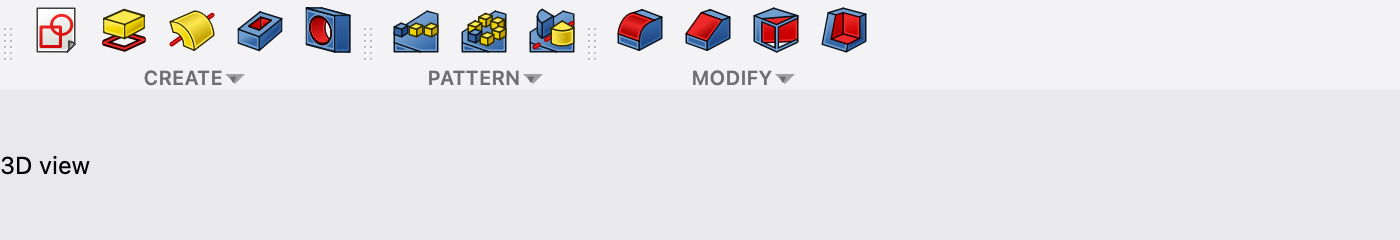
\includegraphics[width=0.62\linewidth]{fig/ui_stepC_caption_proto.png}\\[6pt]
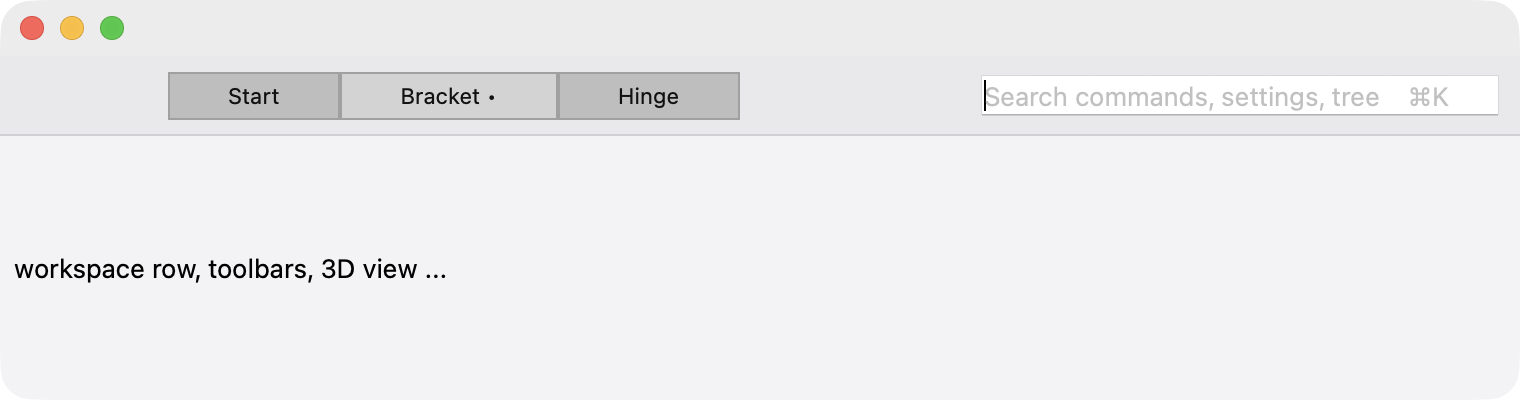
\includegraphics[width=0.80\linewidth]{fig/ui_stepC_titlebar_proto.png}
\caption{Feasibility prototypes, Qt~6.8.3 from this build's environment, FreeCAD's icons. \emph{Top (C1):} captions
as a child button in a 14\,px bottom margin of a plain \code{QToolBar}, drawn offscreen. \emph{Bottom (C4):} a real
window on this Mac after the three \code{NSWindow} calls made from Python through \code{ctypes}. The Qt content
now fills the frame under the traffic lights. In this first run the row still sits below the 28\,pt safe area.
With \code{WA\_ContentsMarginsRespectsSafeArea} off it moves to $y = 0$.}
\label{fig:stepC-proto}
\end{figure}

%----------------------------------------------------------------------
\subsubsection*{C5. Start page}

\textbf{What you see.} The mock's Start page (figure~\ref{fig:ui-sketch-start}, bottom). On the left: \emph{New}
(Part, Assembly, Drawing, Sketch, Simulation study), \emph{Open}, and the vault summary. On the right: recent
files as cards, then as a table with part number, revision, state, date and location. At the foot are the
examples and \emph{Show this page at startup}.

\textbf{How it is built.} FreeCAD's Start page is the C++ \code{StartGui::StartView}, an MDI view whose content is
a \code{QStackedWidget}. Page~0 is the first-start page and page~1 the documents page
(\file{Mod/Start/Gui/StartView.cpp:68, 100--104}), chosen once at \file{:183}. \file{bruceworx\_start.py}
finds the view by name (\code{findChild<StartView*>("StartView")}, as \file{Manipulator.cpp:57} does). It adds
the BruceWorx page as page~2 and selects it. It does this again whenever \code{Start\_Start} re-creates the view,
which it notices through \code{QMdiArea::subWindowActivated}. The view keeps its tab, its close behaviour and
\code{ShowOnStartup} (\file{AppStartGui.cpp:83}). The page itself is plain Qt widgets styled by the token sheet:
\begin{itemize}[nosep]
  \item \emph{New} buttons run the existing commands (\code{Std\_New}, then the part or assembly template).
  \item \emph{Recent} reads \code{BaseApp/Preferences/RecentFiles} (\code{MRU0}\ldots). Thumbnails come from
        \file{thumbnails/Thumbnail.png} inside the \file{.FCStd} zip.
  \item \emph{P/N, revision, state} come from the part properties (\S\ref{sec:partprops}) in the file's
        \file{Document.xml}, or from the folder vault's journal when the file is in a vault
        (\S\ref{sec:pdm-decision}). Both are read on a worker thread and cached by modification time.
  \item \emph{Vault summary} (checked out, waiting for review, released this week) comes from the vault. Until
        \eref{PDM-04} exists the box says ``No vault open'' and links to opening one.
\end{itemize}
\emph{C++ alternative:} rewrite \code{StartView}'s layout with \code{[BW]} changes. The Start module was rewritten
for 1.0 and still changes, so it is not recommended.

\textbf{Effort:} 2--3 days, of which the vault part depends on \eref{PDM-04}. \textbf{Risks:}
\begin{itemize}[nosep]
  \item \code{StartView} switches pages itself when the first-start page is opened or dismissed
        (\file{StartView.cpp:429, 438}). The module must re-select page~2 after that.
  \item Parsing many large \file{.FCStd} files must not block the UI. A worker thread and a cache by
        modification time handle this.
  \item An upstream change to \code{StartView}'s object name or page stack would break the lookup. A test checks
        for it.
\end{itemize}

%----------------------------------------------------------------------
\subsubsection*{Summary and recommended order}

\begin{center}
\small
\begin{tabularx}{\linewidth}{@{}lXllll@{}}
\toprule
\# & Item & Where & Effort & Upstream risk & macOS only\\
\midrule
C1 & Captioned groups & Python & 1--2 d & none & no\\
C2 & Workspace menu and tabs & Python + json & 3--4 d & none (command renames) & no\\
C3 & Search, \texttt{Cmd-K} & Python & 2 d & none & no\\
C4 & Tabs in the title bar & Python \code{ctypes} (or one \file{.mm}) & 2--3 d & none (or low) & yes\\
C5 & Start page & Python in \code{StartView} & 2--3 d & low & no\\
\midrule
 & Total & & 10--14 d & & \\
\bottomrule
\end{tabularx}
\end{center}

\textbf{Order: C1 $\rightarrow$ C2 $\rightarrow$ C3 $\rightarrow$ C4 $\rightarrow$ C5.}
\begin{itemize}[nosep]
  \item C1 is small, stands alone and changes the most visible thing. C2 needs its caption button.
  \item C2 is the biggest gain and fixes the group and command lists that C3 searches.
  \item C3 needs a place in the title row but works in the step B row too, so it can come before C4.
  \item C4 is macOS-only polish on top of step B's tabs. It is the riskiest, and the fallback already works.
  \item C5 is the least coupled, and its vault part waits for \eref{PDM-04} anyway.
\end{itemize}
Each item ends like steps A and B: the four screens captured from the real build, light and dark, next to these
mocks, plus tests for the pure logic. These are json validation, the tab model, search ranking and the
recent-file parsing.

%----------------------------------------------------------------------
\subsubsection*{Questions before step C starts}

\begin{enumerate}
  \item \textbf{Search.} Is the built-in \texttt{Cmd-K} field (C3) what you meant by ``yes'', rather than the
        SearchBar add-on restyled?\\
        \emph{Recommendation:} built-in; SearchBar stays installed and is hidden while the field is on.
  \item \textbf{Python instead of a C++ \code{WorkspaceSelector}.} On 18 Oct this was planned as C++ work on the
        workbench selector. Is it fine to build the workspaces in Python on stock FreeCAD (custom toolbars,
        manipulator, observers) as described in C2?\\
        \emph{Recommendation:} yes. It has no upstream conflicts for the rebase, and every part can be
        switched off.
  \item \textbf{An assembly document in Design.} Should Design stay on the Part Design workbench, with the
        assembly tools in \textsc{Solid $\rightarrow$ Assemble}? Or should it switch the underlying workbench
        to Assembly whenever an assembly document is active? The label stays \textsc{Design} either way. The
        second keeps the Assembly workbench's own context menu and task-panel watchers, at the cost of a
        toolbar rebuild when you change document tabs.\\
        \emph{Recommendation:} stay on Part Design and add the Assembly context-menu items through the
        manipulator. Change this if it feels wrong in use.
  \item \textbf{Tabs in Simulation, Manufacture and Drawing.} Should they start with one tab each (the
        workbench's own toolbars as captioned groups), or get Fusion-like tabs now (Simulation: Setup,
        Solve, Results; Manufacture: Setup, Milling, Utilities)?\\
        \emph{Recommendation:} one tab each in step C, with Fusion-like tabs as part of \eref{SIM-01} and the
        CAM work, when those workspaces get real use.
  \item \textbf{Where workbenches are shown or hidden.} Should the ticks in figure~\ref{fig:stepC-prefs} write
        FreeCAD's own enabled-workbench list, so a hidden workbench is not loaded at all? Or should they keep
        a separate Vector Labs list that only hides it from the menu?\\
        \emph{Recommendation:} write the stock list. There is one truth, and start-up is faster.
  \item \textbf{Title bar route.} For C4, should the native calls stay in Python via \code{ctypes} (no
        compiled code, no upstream diff), or go in a small \file{MacTitleBar.mm}? And should the row be
        40\,px with the traffic lights centred by an empty compact \code{NSToolbar}?\\
        \emph{Recommendation:} \code{ctypes} first, and a 40\,px row as in the mock. If the lights cannot be
        centred cleanly, use a 28\,pt row (smaller tabs) rather than moving the buttons by hand.
  \item \textbf{Start page.} Should the BruceWorx page replace the stock page's content inside the existing
        Start tab (the stock page stays reachable when the switch is off)? And before a vault exists, should
        the left column show the vault box with ``No vault open'', or hide it?\\
        \emph{Recommendation:} replace the content, and show the box with an \emph{Open vault\ldots}
        link, so the vault is easy to find.
  \item \textbf{Group contents.} Should the groups come only from \file{workspaces.json} in step C, with the
        caption menu's \emph{Pin to toolbar\ldots} (move a command between the row and the menu) left for
        later?\\
        \emph{Recommendation:} yes. Editing your own groups needs a small editor and conflicts with Tools
        $\rightarrow$ Customize, so it should be a separate decision.
  \item \textbf{Fusion single-key shortcuts.} Should step C add shortcuts like \texttt{S} (sketch),
        \texttt{E} (pad/extrude) and \texttt{H} (hole), as listed in the \textsc{Create} menu of
        figure~\ref{fig:stepC-groups}? Some single keys are taken in sketch edit mode.\\
        \emph{Recommendation:} not in step C. Show FreeCAD's existing shortcuts only, and decide on a Fusion
        key map together with the command-line aliases (\eref{AUT-05}).
\end{enumerate}
